\documentclass{article}

\usepackage[english]{babel}
\usepackage[utf8]{inputenc}
\usepackage{amsmath,amssymb}
\usepackage{parskip}
\usepackage{graphicx}
\usepackage{listings}
\usepackage{float}
\lstset{
    numbers=left, 
    numberstyle= \tiny, 
    keywordstyle= \color{ blue!70},
    commentstyle= \color{red!50!green!50!blue!50}, 
    frame=shadowbox, % 阴影效果
    rulesepcolor= \color{ red!20!green!20!blue!20} ,
    escapeinside=``, % 英文分号中可写入中文
    xleftmargin=2em,xrightmargin=2em, aboveskip=1em,
    framexleftmargin=2em,
    breaklines=true,
    language=python
} 
% Margins
\usepackage[top=2.5cm, left=3cm, right=3cm, bottom=4.0cm]{geometry}
% Colour table cells
\usepackage[table]{xcolor}


% Get larger line spacing in table
\newcommand{\tablespace}{\\[1.25mm]}
\newcommand\Tstrut{\rule{0pt}{2.6ex}}         % = `top' strut
\newcommand\tstrut{\rule{0pt}{2.0ex}}         % = `top' strut
\newcommand\Bstrut{\rule[-0.9ex]{0pt}{0pt}}   % = `bottom' strut

%%%%%%%%%%%%%%%%%
%     Title     %
%%%%%%%%%%%%%%%%%
\title{CSCI803 ASS2}
\author{Name: Yao Xiao \ SID: 2019180015}
\date{\today}

\begin{document}
\maketitle

%%%%%%%%%%%%%%%%%
%   Problem 1   %
%%%%%%%%%%%%%%%%%
\section{Sentiment Analysis}
\subsection{Describe the procedure of collecting the tweets and manually tagging them}
We apply for consumer key and access token calls twitter API to get tweets related to Hate speech topics (like racist and sexism), and classifies related emotions with textblob, converts the data into correct input format, and classifies users' views into positive (non racist) and negative (racist) by tweeting. 
The specific algorithm is as follows:
\begin{lstlisting}
import tweepy
from textblob import TextBlob

api = tweepy.API(auth
public_tweets = api.search('hate',lang="en")
for tweet in public_tweets:
  print(tweet.text)
  analysis = TextBlob(tweet.text)
  print(analysis.sentiment)
  if analysis.sentiment[0]>0:
    print("positive")
  elif analysis.sentiment[0]<0:
    print("negative")
  else:
    print("neutral")
\end{lstlisting}


\subsection{Describe the statistics of the obtained data set}
From the obtained the data, we can see the shape of train data is (31962, 3),
the shape of test data is (10655, 2).

And the train data has two label, 0 and 1. Among them, the size of label-0 is 29720,
and the size of label-1 is 2242, the data format is as follows:

\begin{figure}[H]
    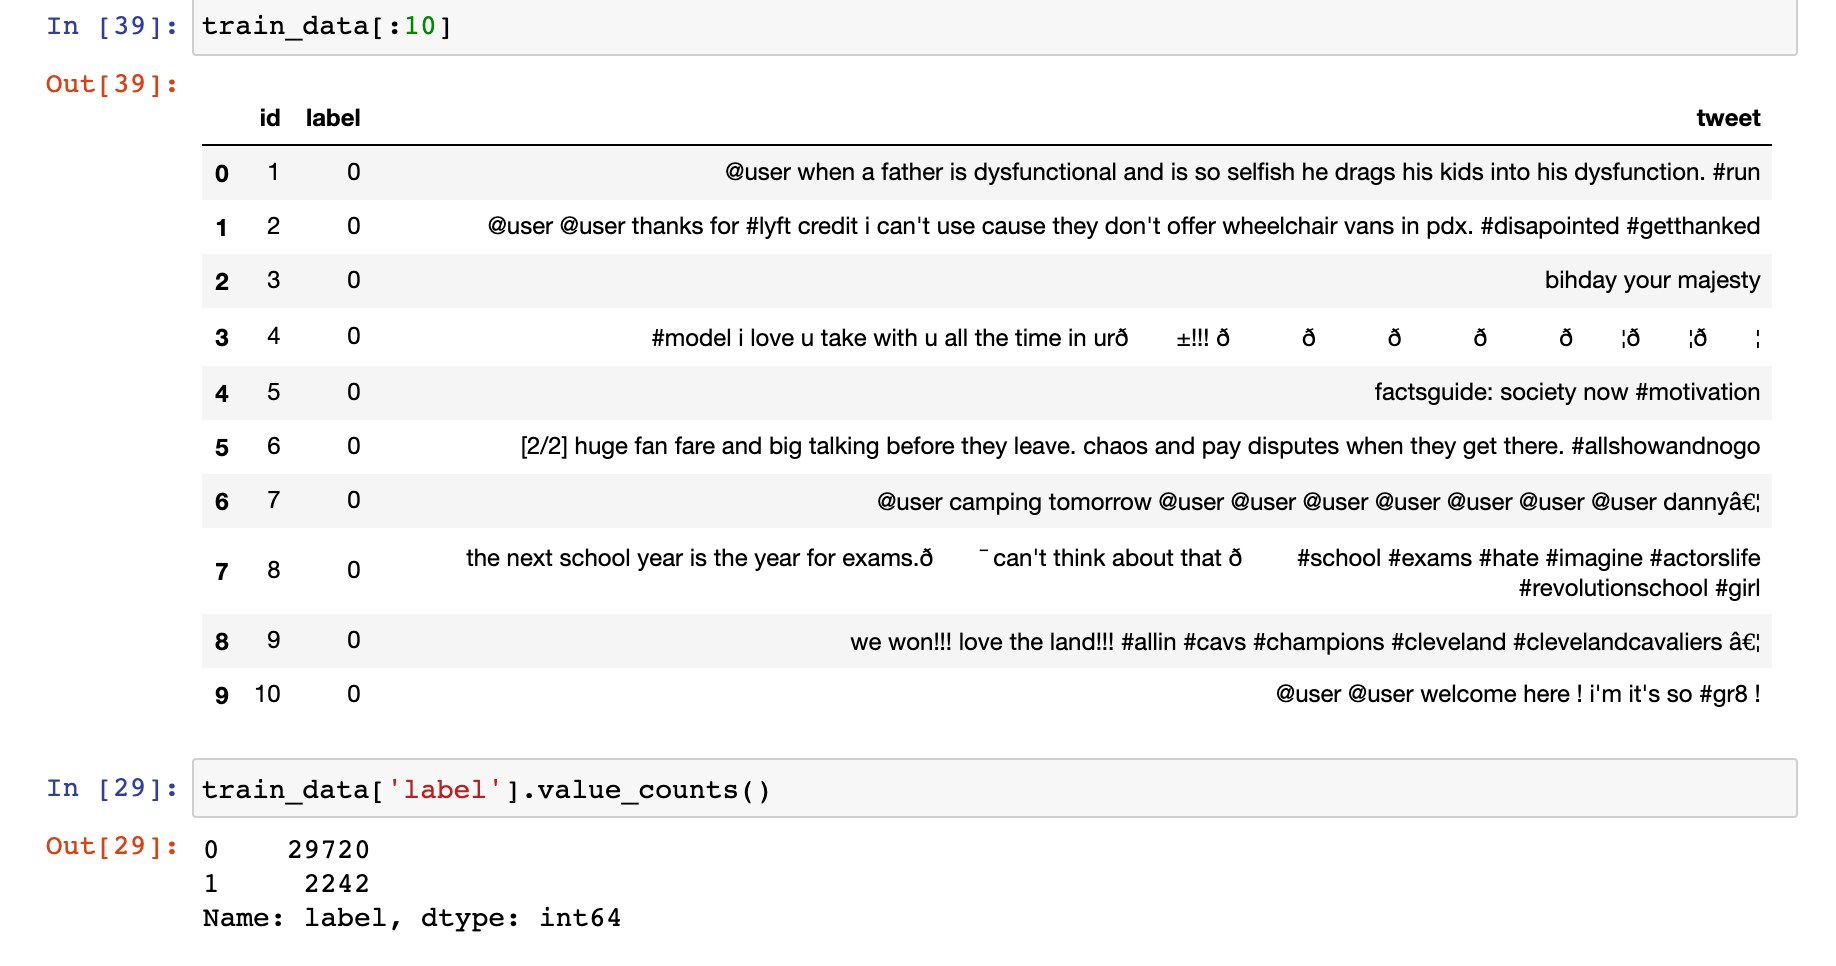
\includegraphics[width=1\textwidth]{Fig1}
\end{figure}

Here is the simple analysis:

\begin{figure}[H]
    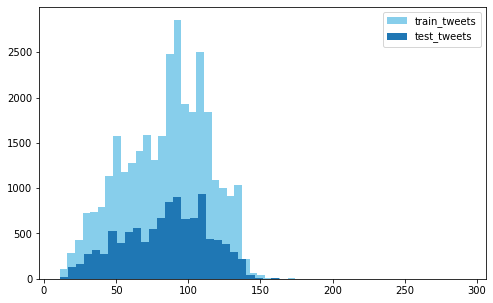
\includegraphics[width=1\textwidth]{Fig2}
\end{figure}

\subsection{Describe how you represent each tweet for classification}

In the beginning, we clear the data and get the pure text for further processing.
For the nlp task, we first should cut a whole sentence into characters or words, also named toeknizing;
and then convert text to index.

Specific to the project, we created a function to create a vector for each tweet by taking the average of the vectors of the words present in the tweet,
and then build the embedding matrix.

And for the pretrained, we choose Word2Vec model.

\begin{figure}[H]
    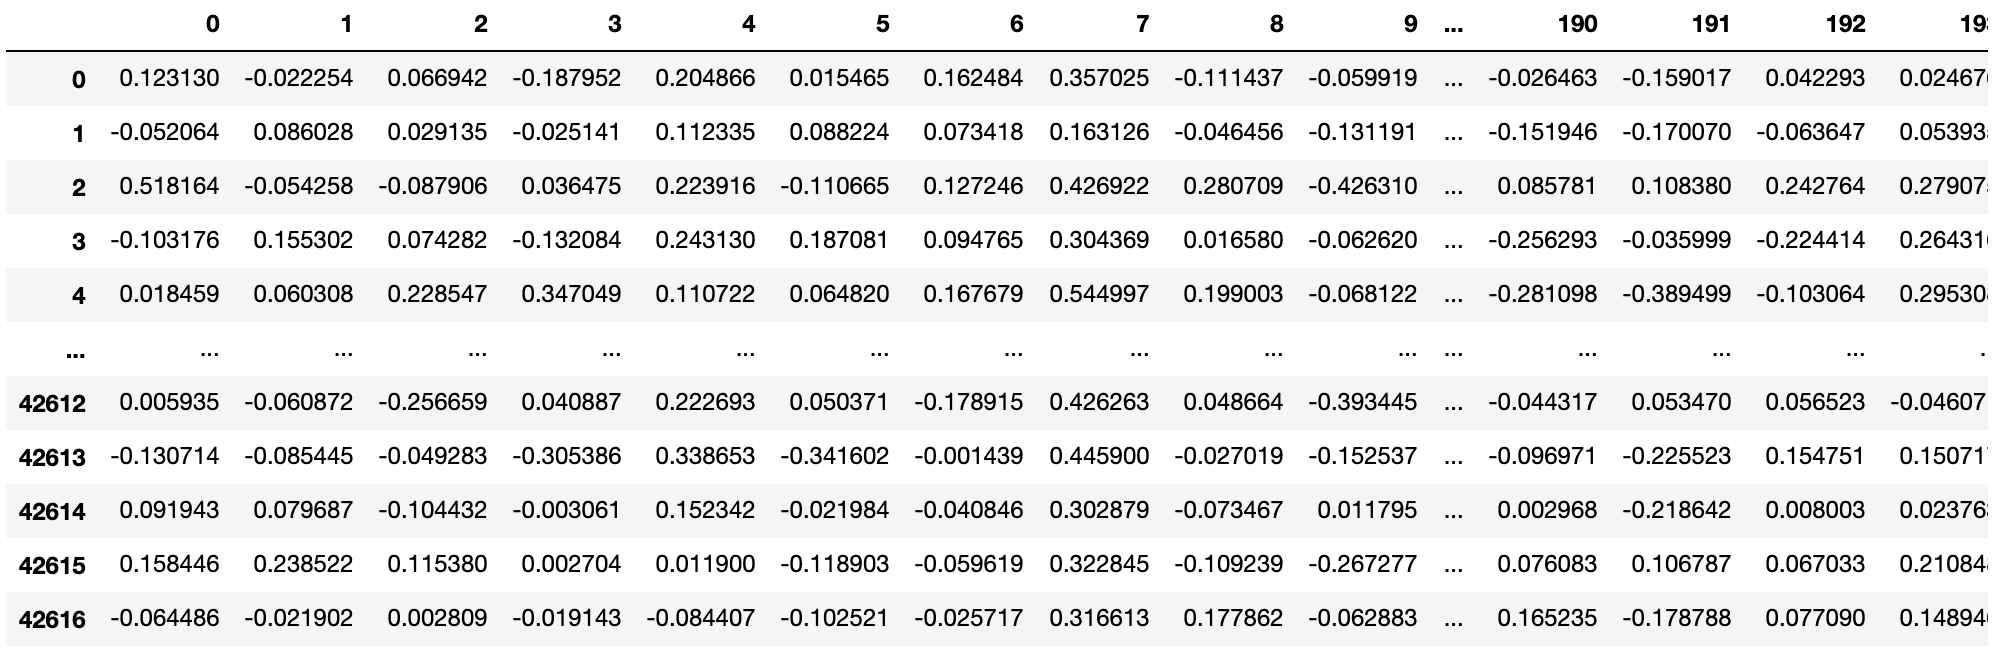
\includegraphics[width=1\textwidth]{Fig3}
\end{figure}

\subsection{For each classifier, describe its working principle, classification procedure, and parameter setting}
\subsubsection{Logistic Regression}

Logistic Regression is a classification algorithm could help us predict whether the given Tweet is Racist or not. Logistic regression predictions are distinct. We can also view probability scores underlying the model's classifications. Logistic regression transforms its output using the logistic sigmoid function to return a probability value which can then be mapped to two or more discrete classes. 

\subsubsection{Naive Bayes}

Naive Bayes is a classification technique based on Bayes' theorem, assuming independence between predictors. Bayes' theorem provides an equation to describe the relationship between conditional probabilities of statistics. In Bayesian classification, we are interested in the probability of finding a label given certain observation characteristics. There are three types of Naive Bayesian models. Gauss, polynomial and Bernoulli. Gaussian is basically used for classification problems, while polynomials are used to obtain different counts. If the feature vector is binary, Bernoulli is used.

\subsubsection{SVM}

SVM is a supervised machine learning algorithm for classification and regression problems. In SVM, we perform classification by finding a hyperplane that can distinguish two categories well. Kernel tricks are used to transform data and then find the best boundary between possible outputs based on the data. Hyperparameters such as kernel, regularization, gamma, and margins can be used to optimize SVM.

Settings as follows:

\begin{lstlisting}
    svc = svm.SVC(kernel='linear', C=1, probability=True)
\end{lstlisting}

\subsubsection{Random Forest}
Random forest is a supervised learning algorithm. It can be used for classification and regression. It is also the most flexible and easy to use algorithm. The forest is composed of trees. It is said that the more trees, the stronger the forest. Random forest creates decision trees on randomly selected data samples, obtains predictions from each tree and selects the best solution through voting.

Settings as follows:

\begin{lstlisting}
    rf = RandomForestClassifier(n_estimators=400, random_state=12)
\end{lstlisting}

\subsubsection{XGBoost}
XGBoost stands for “Extreme Gradient Boosting”, where the term “Gradient Boosting” originates from the paper Greedy Function Approximation: A Gradient Boosting Machine, by Friedman.
\begin{equation}
    \mbox{Prediction: } \ \hat{y}^{t}_i = \hat{y}^{t-1}_i + f_t(x_i) 
\end{equation}

\begin{equation}
    \mbox{Loss: } \ \sum^{n}_{i=1} \ell(y_i,\hat{y}^{t-1} + f_t(x_i) ) + \Omega(f_t)
\end{equation}

The working process of XGBoost is that it combines predictions from multiple decision trees. All weak learners in the gradient boosting machine are decision trees. The trees in XGBoost are constructed sequentially, trying to correct the errors of the previous tree.

Settings as follows:
\begin{lstlisting}
    xgb = XGBClassifier(max_depth=6, n_estimators=1000, nthread= 3)
\end{lstlisting}

\subsection{For each classifier, report the classification accuracy, AUC, and plot the confusion matrix}
\subsubsection{Logistic Regression}
\begin{figure}[H]
    \centering
    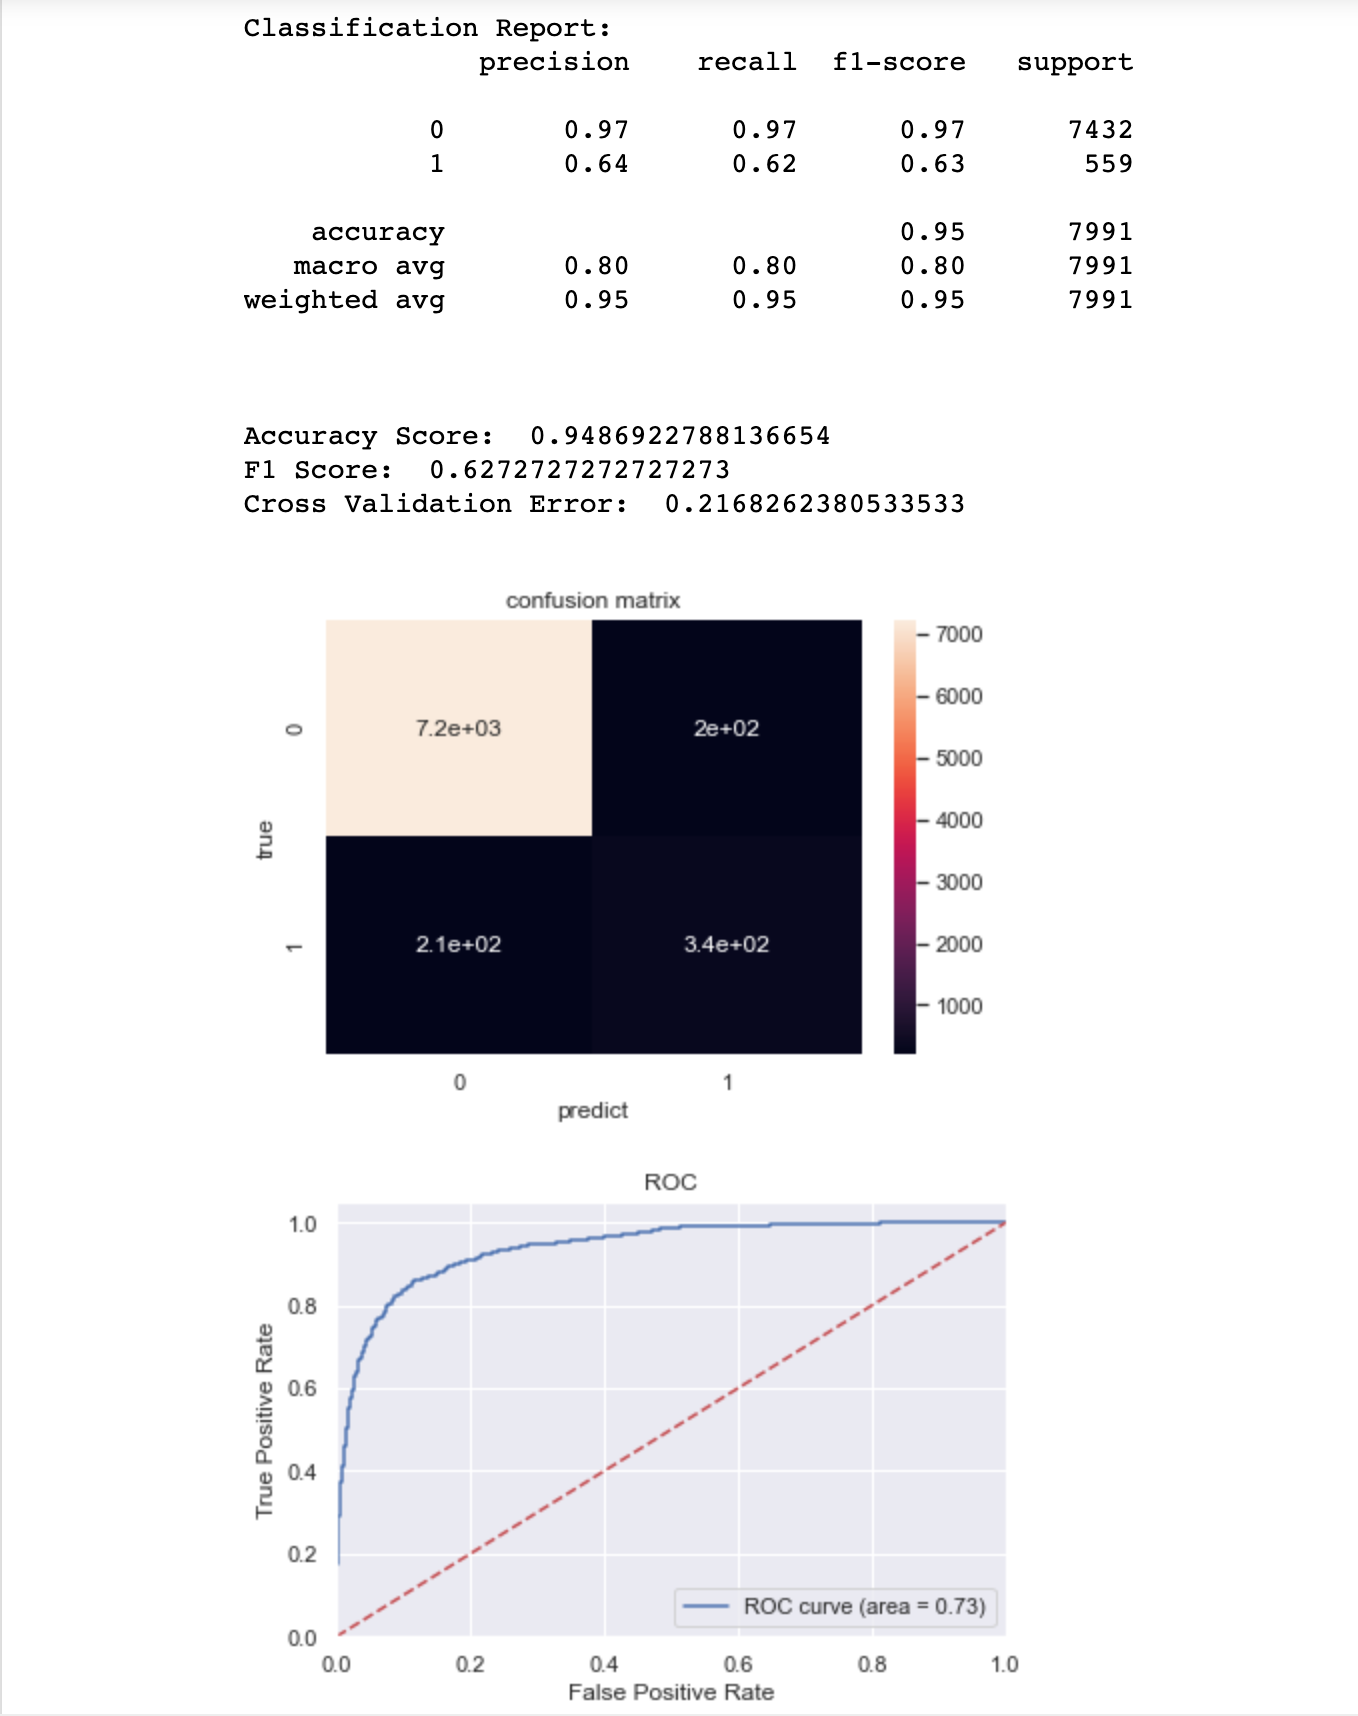
\includegraphics[width=0.85\textwidth]{Fig4}
\end{figure}

\subsubsection{Naive Bayes}
\begin{figure}[H]
    \centering
    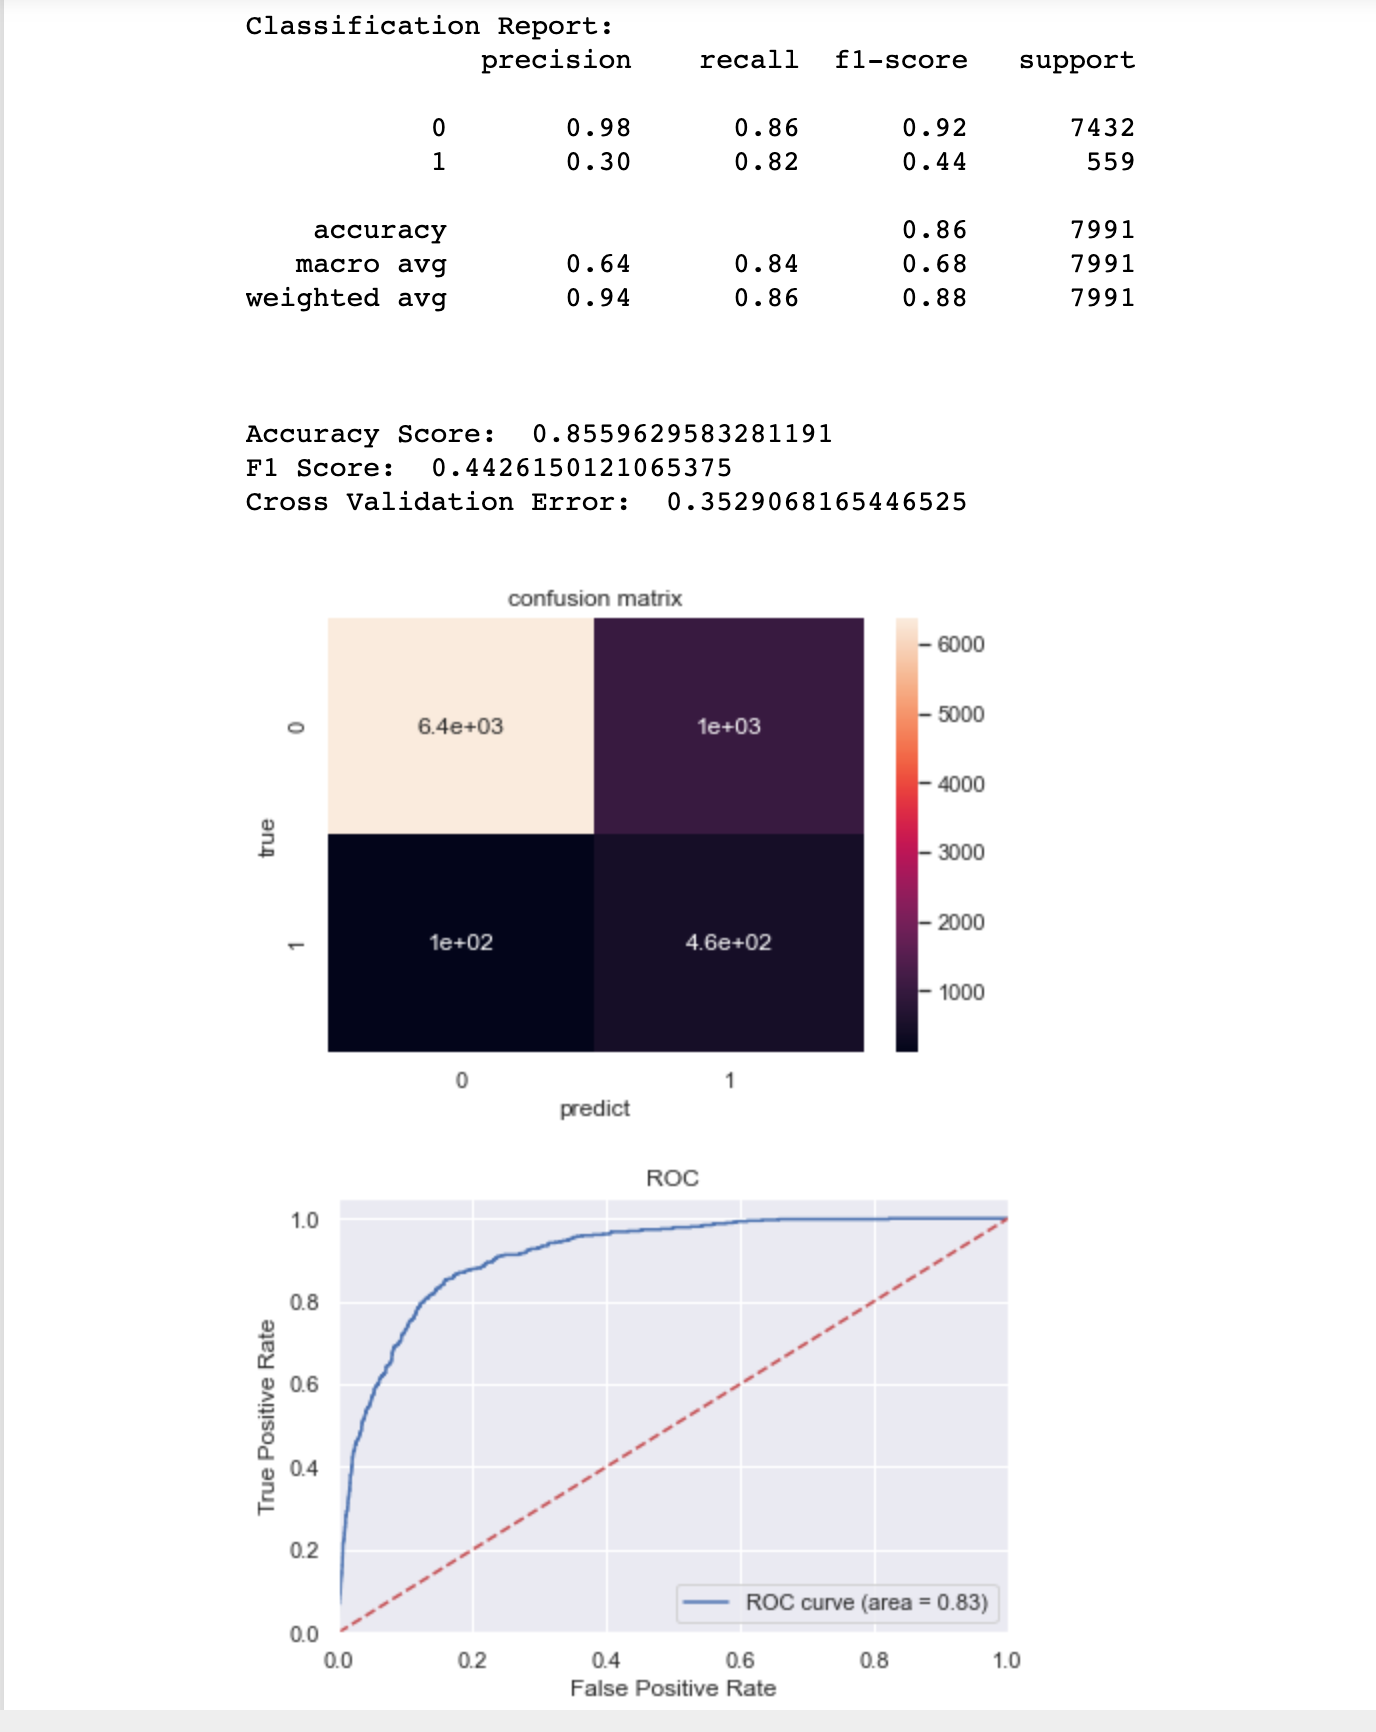
\includegraphics[width=0.85\textwidth]{Fig5}
\end{figure}

\subsubsection{SVM}
\begin{figure}[H]
    \centering
    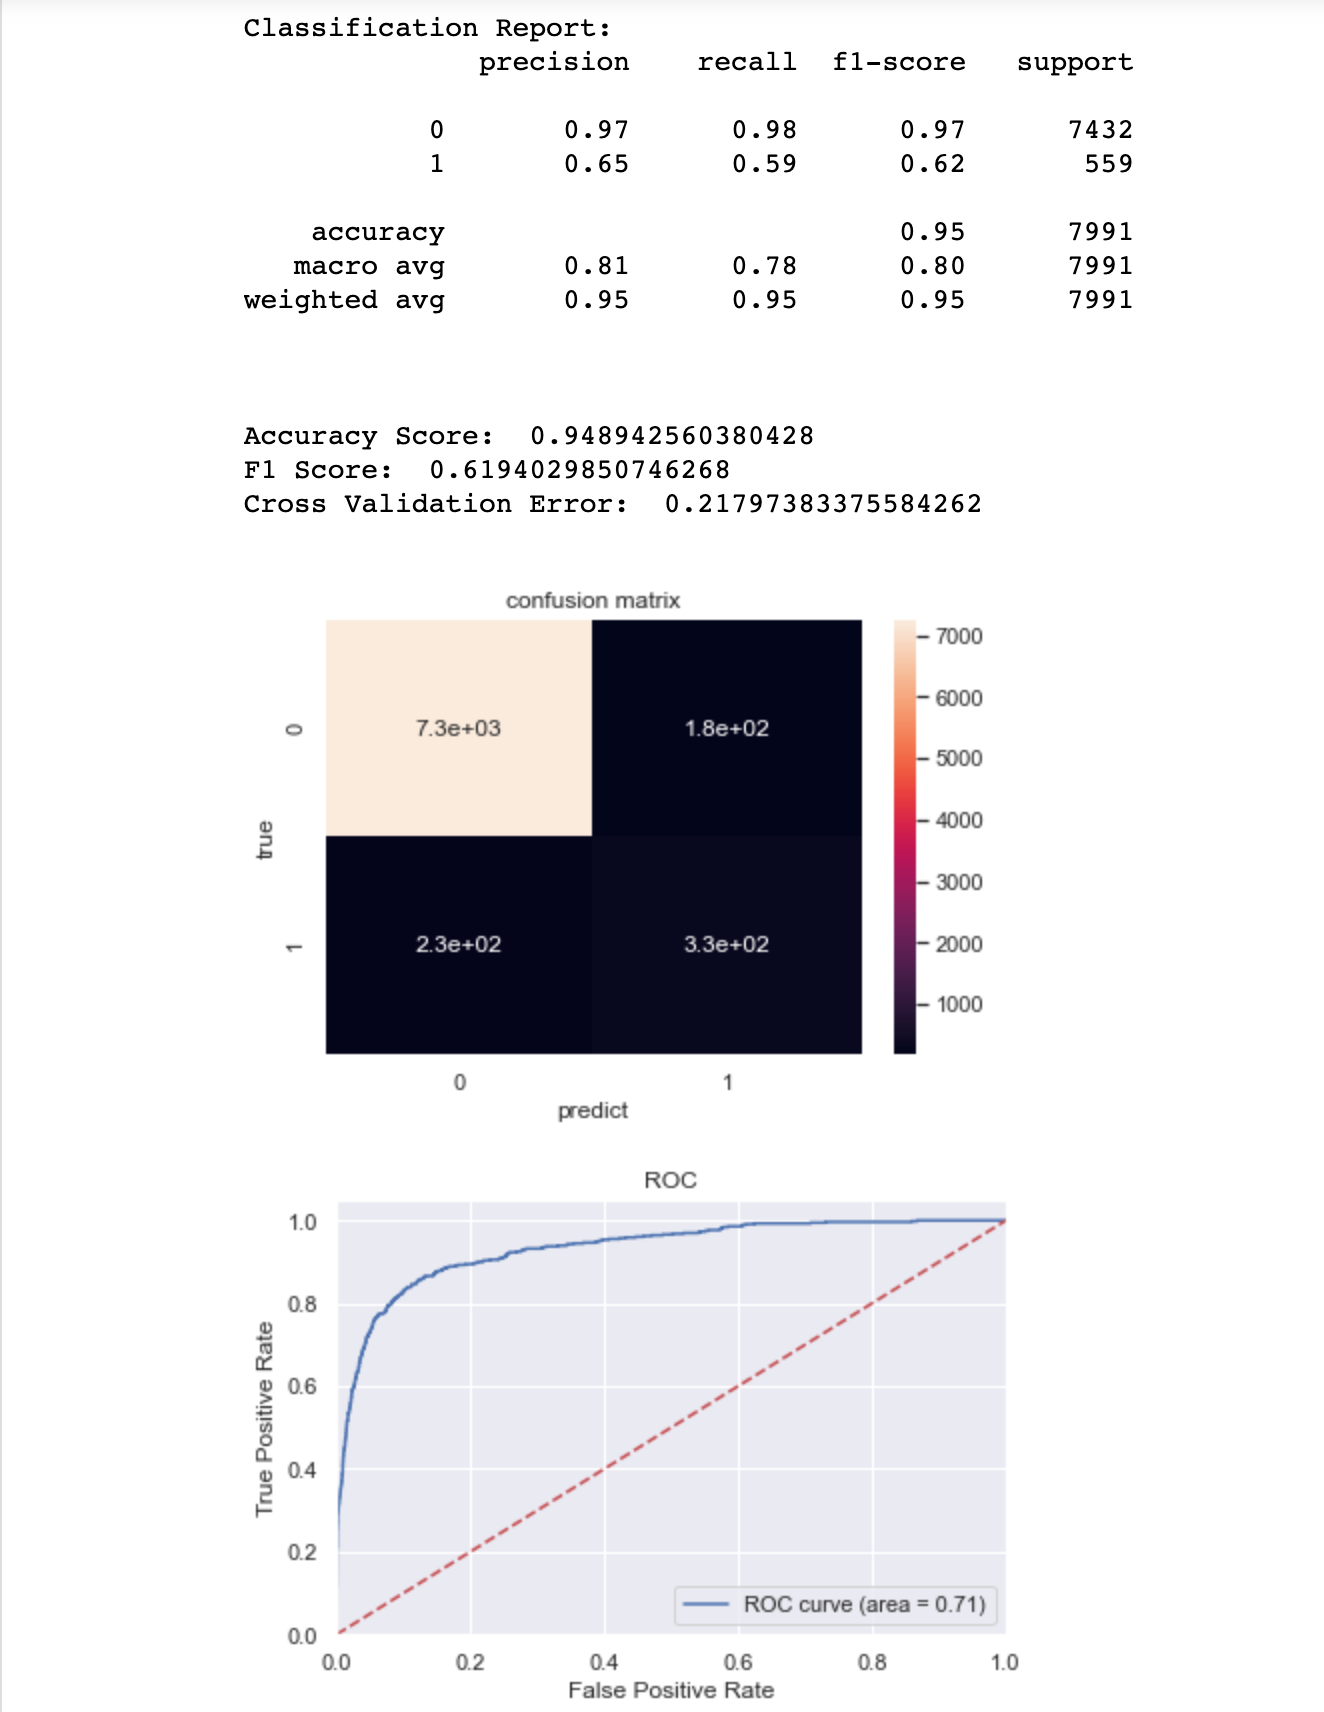
\includegraphics[width=0.85\textwidth]{Fig6}
\end{figure}

\subsubsection{Random Forest}
\begin{figure}[H]
    \centering
    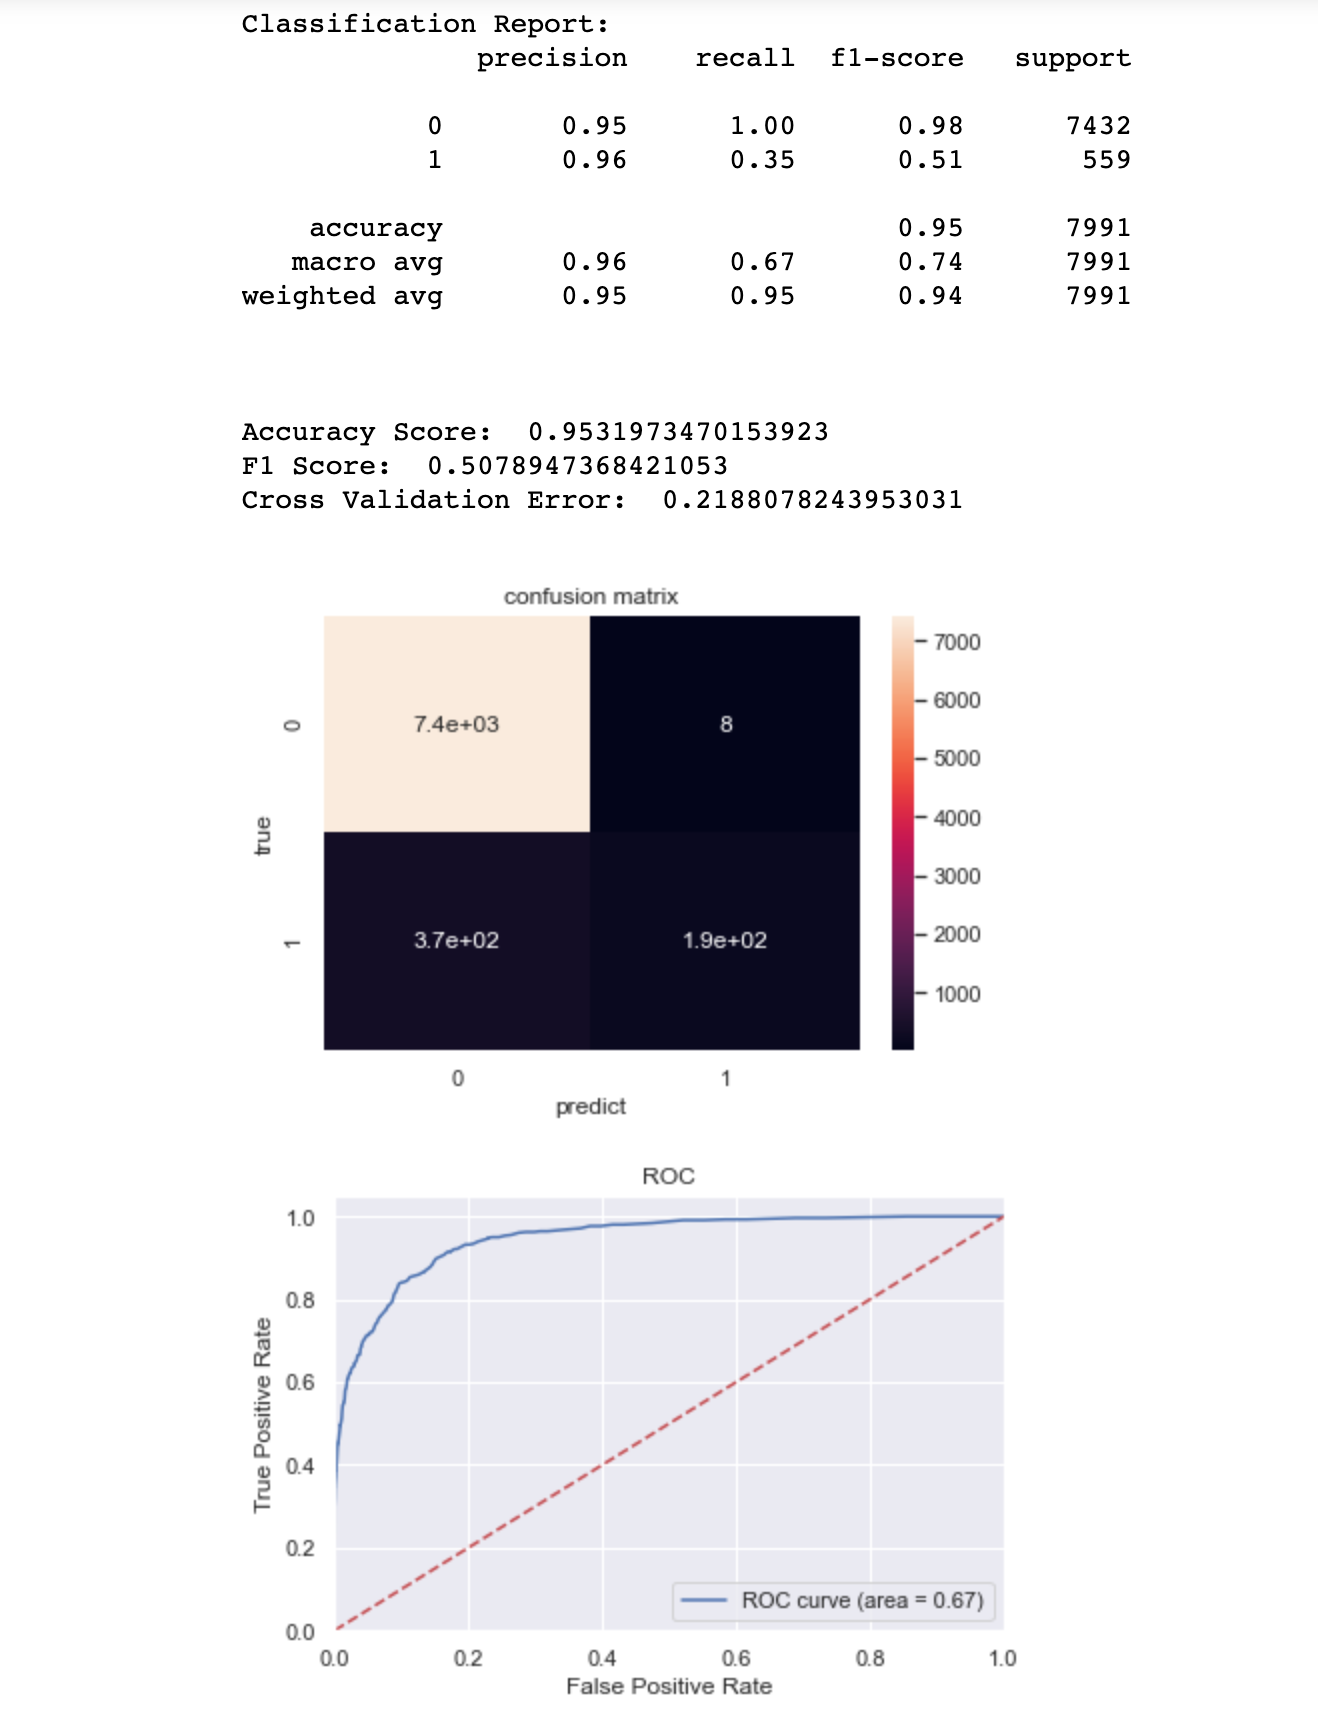
\includegraphics[width=0.85\textwidth]{Fig7}
\end{figure}

\subsubsection{XGBoost}
\begin{figure}[H]
    \centering
    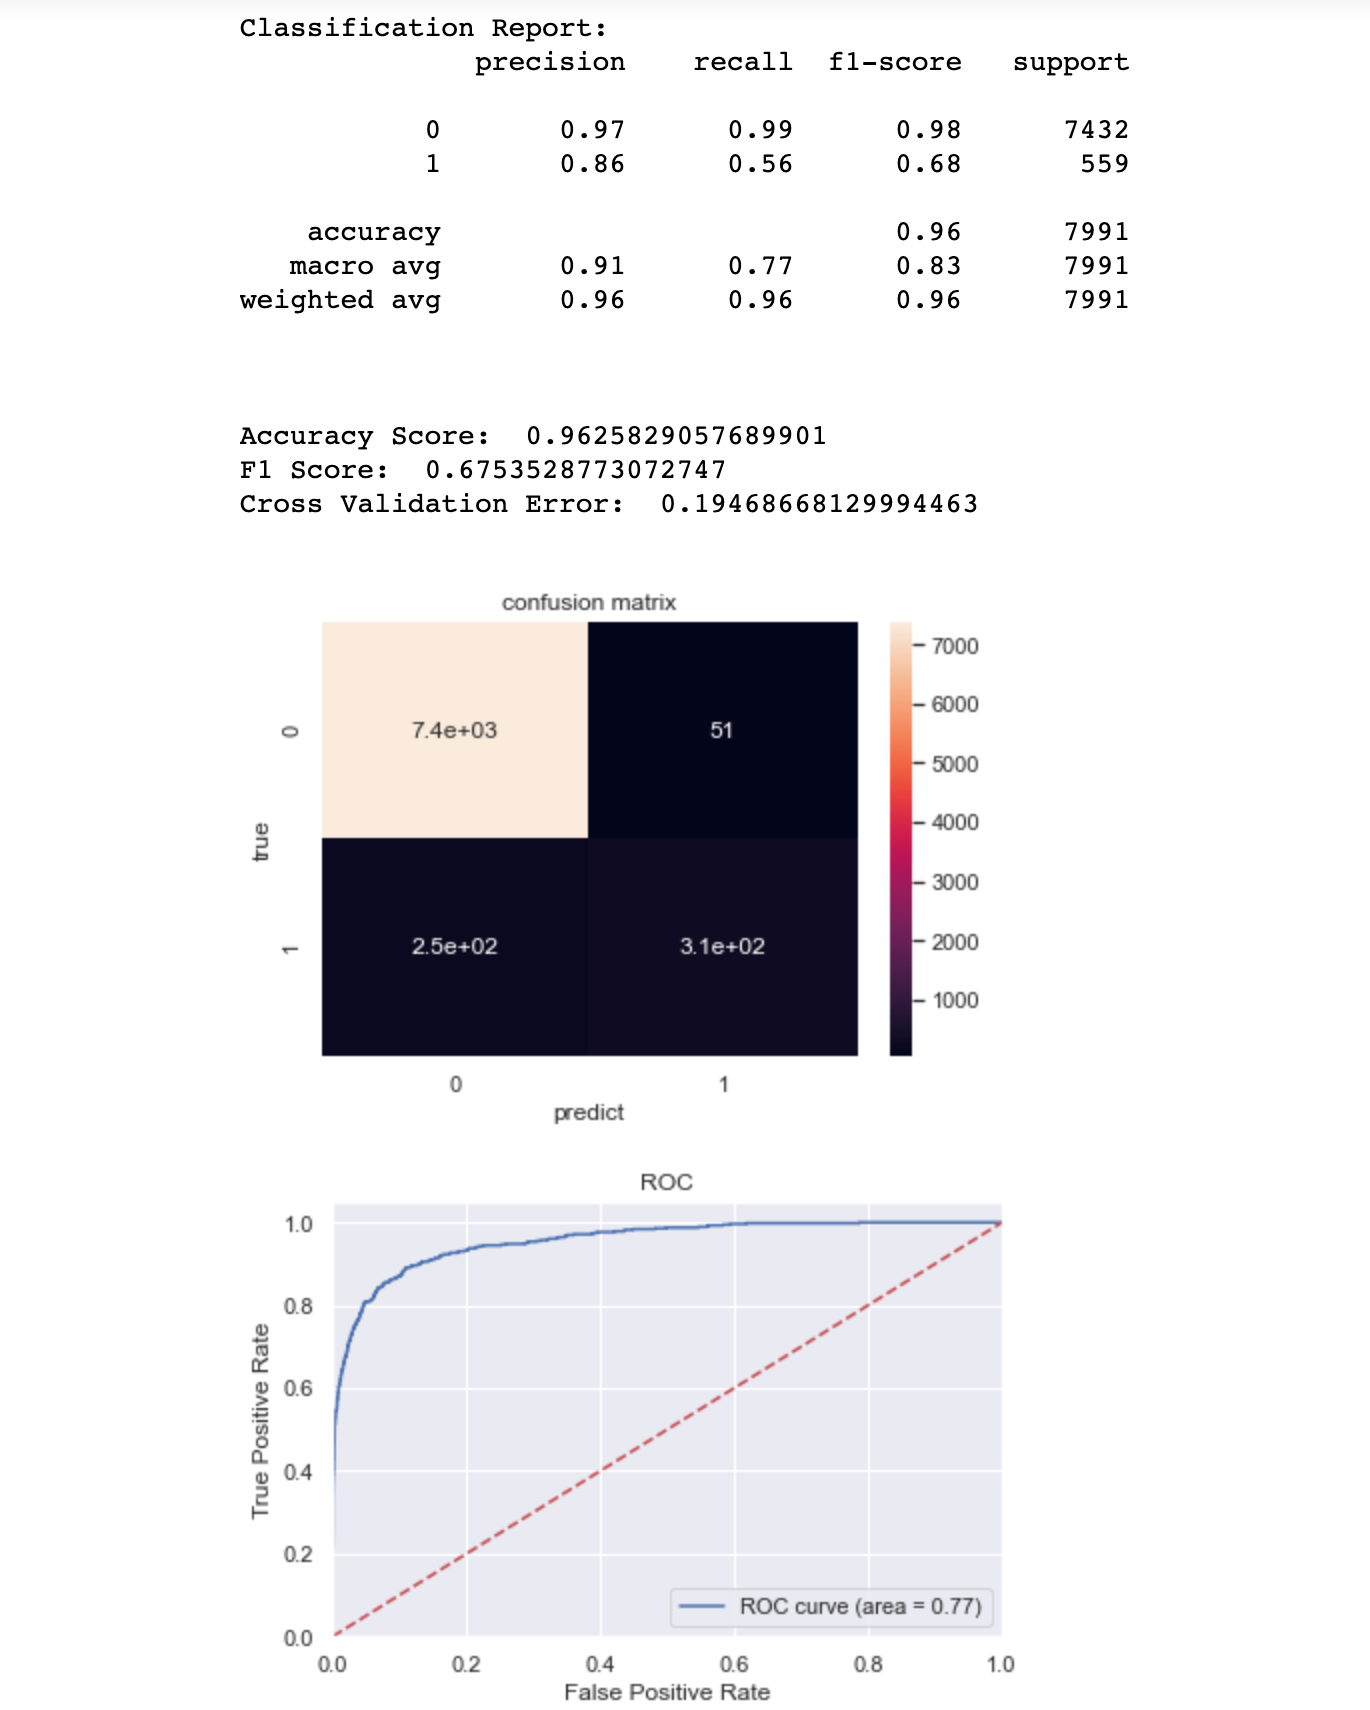
\includegraphics[width=0.85\textwidth]{Fig8}
\end{figure}



\subsection{Report which classifier performs better than the others and describe the methods you use to reach this conclusion}
\begin{figure}[H]
    \centering
    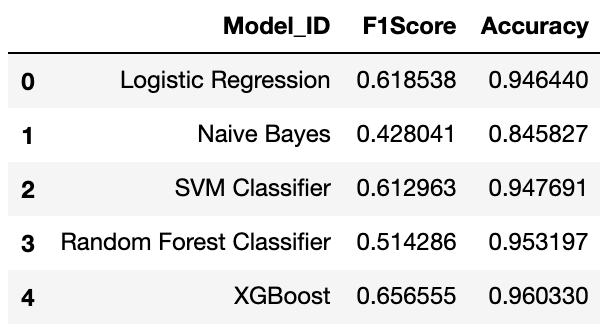
\includegraphics[width=1\textwidth]{Fig9}
\end{figure}

In the unified use of Word2Vec for word embedding, models such as Logistic regression, SVM, Random Forest and XGBoost were evaluated respectively. Combining all evaluation indicators, focusing on F1 scores, we believe that the best performing model is XGBoost, with an F1 score of 0.656.

\end{document}